%si tu veux une équation directement dans le texte c'est $ equation $
%si tu veux une equation seule c'est 
%begin{equation} 
%ton equation 
%end{equation}

\documentclass[a4paper,11pt]{article}
\usepackage[T1]{fontenc}
\usepackage[utf8]{inputenc}
\usepackage{lmodern}
\usepackage[francais]{babel} 
\usepackage[ portrait, margin = 0.7 in]{geometry}   %pour avoir plus de marge

\usepackage{amsmath}      %des trucs de maths en plus
\usepackage{amssymb}	  %pour avoir plus de symboles mathématiques

\usepackage{mathrsfs}  
\usepackage{dutchcal}
\usepackage{graphicx}

\graphicspath{{./images/}}    %dir de tes images

%Les deux suivants servent à faire des sous figures dans les figures avec leur propre légende
\usepackage{float}			  
\usepackage{subfig}

\usepackage{gensymb}
\usepackage{makecell}
\usepackage{bm}     %pour avoir du texte en gras dans les équations \bm{truc_en_gras}
\numberwithin{equation}{section}

\DeclareMathOperator{\arccosh}{arccosh}  %si tu veux créer des nouveaux opérateurs de math

\begin{document}  

\title{\LARGE \bf Évaluation du Code de caractérisation d'amas PROF-CL}
\author{MERCIER Wilfried - Observatoire de Paris}
\maketitle

\newpage  %forcer latex à commencer une nouvelle page

\section{Notations utiles}  %nouvelle section (numerotation auto)

\begin{tabular}{l l l}   %tableau {l l l} veut dire trois colonnes où le texte est aligné à gauche à chaque fois
  Nom & Symbole(s) & Description \\   %le & dit les endroits où latex doit aligner et le \\ la fin de ligne
  Profil NFW & $\bm{\rho_{NFW}}$ & Profil de densité universel de matière noire Navarro, Frenk, White \\
  Rayon de pente -2 &  $\bm{r_s$} , \bm{$r_{-2}}$ & Rayon pour lequel la pente de $\rho_{NFW}$ vaut -2 \\
  & $\bm{r_{200}}$ & Rayon pour lequel la densité de la sphère vaut 200 fois la densité \\
  & & moyenne de matière dans l'Univers \\
  Rayon viriel & $\bm{r_{vir}}$ & Rayon pour lequel la matière dans la sphère est en équilibre
\end{tabular}

\newpage

\begin{figure}              %pour mettre une image
  \label{Median_separation}      %label que tu peux appeler avec ref{label} où label est le nom donné, ça donne automatique un numero à ta section/equation/figure, etc... sans avoir à te soucier du numéro
	\begin{center}      %centrer ton image
		\subfloat[Biais sur le logarithme du rayon caractéristique en fonction du nombre de galaxies. Les valeurs médianes et moyennes sont légèrement décalées pour des questions de visibilité. On remarque que la séparation médiane se comporte assez bien à nombre de galaxies élevé.]{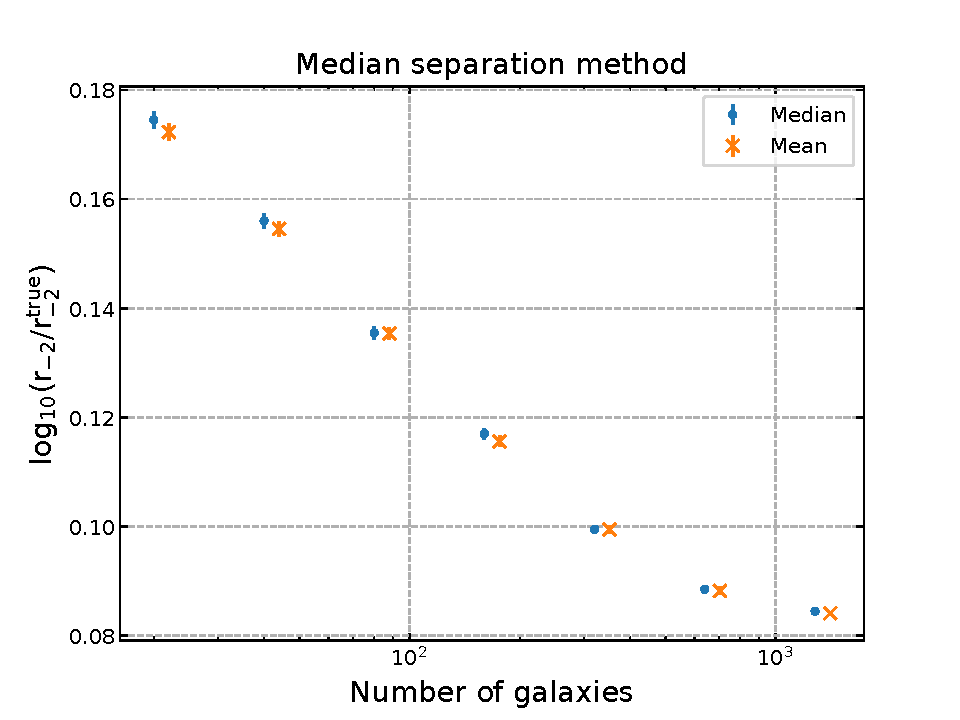
\includegraphics[scale=0.48]{mediansep.pdf}}      %une sous-figure de taille 0.48 la largeur de la page où le texte entre [] est la description de la sous-figure et {mediansep.pdf} est le nom
		\quad  %ajoute un espace
		\subfloat[Dispersion sur le logarithme du rayon caractéristique. Comme pour le biais on remarque que la dispersion diminue avec le nombre croissant de galaxies.]{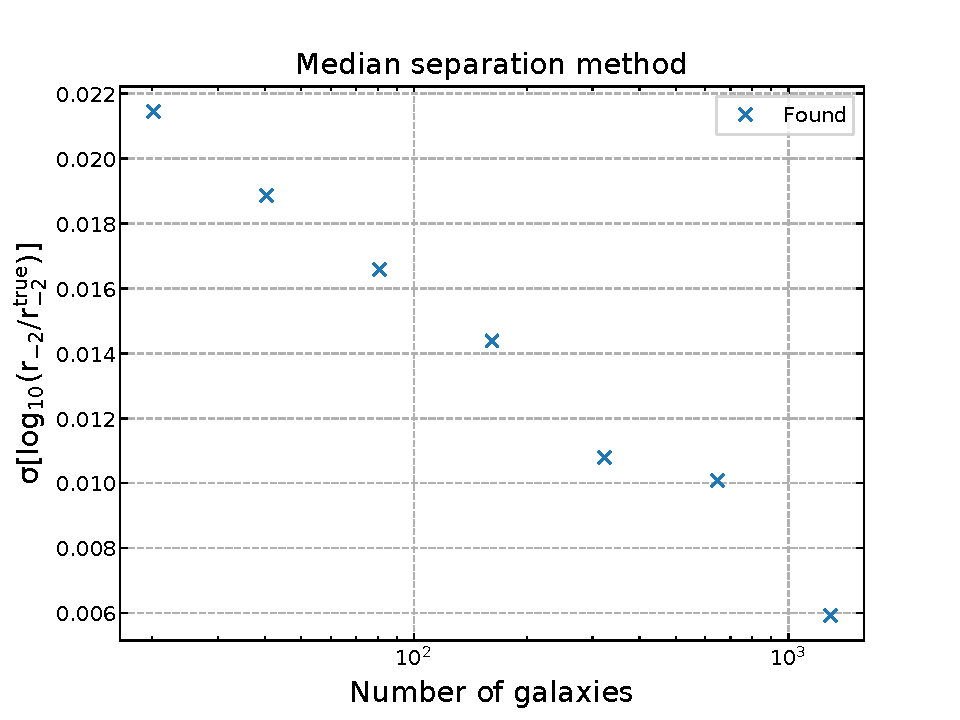
\includegraphics[scale=0.48]{medsep_scat.pdf}}   %seconde figure
	\end{center}
	\caption{Biais et dispersion pour la séparation médiane. Chaque valeurs est calculée pour 100 itérations d'amas d'Emmanuel ARTIS contenant 20, 40, 80, 160, 320, 640 et 1280 galaxies.}  %description de la figure complete
	\label{fig:Median}
\end{figure}

  \section{Séparation médiane}
    En plus des méthodes d'optimisation par maximum de vraisemblance on peut obtenir des résultats similaires en considérant cette fois la séparation médiane entre les galaxies.\newline %retour a la ligne
    Si l'on possède un ensemble de N galaxies alors on aura $N(N-1)/2$ séparations du type $\Delta l_{kl} = \vert l_k - l_l \vert$. On obtient alors une matrice symétrique sur laquelle on peut calculer la séparation médiane sur la partie triangulaire haute par exemple.\newline
Comme on peut le voir sur la Figure \ref{fig:Median} la méthode fournit des résultats corrects avec une erreur relative de l'ordre de $20\%$ lorsqu'on approche $10^3$ galaxies par amas.
  \newpage
  
  \section{Halo de matière noire : Profil NFW et surface de densité}
  \subsection{Profils NFW et NFW tronqués}
    Vers la fin des années 1990 Navarro, Frenck et White montrèrent à l'aide de simulations numériques à N-corps que les halos de matière noire formés dans des cosmogonies de type CDM possèdent deux caractéristiques universelles:
    
    \begin{itemize}    %liste
      \item ils suivent tous un profil de densité NFW
      \item ils sont isotropes
    \end{itemize}

    La seconde propriété n'est cependant vraie que dans le cas de halos de matière noire sphériques. Le profil NFW est généralement écrit sous la forme\cite{NFW1996}
    
    \begin{equation}
      \label{eq:NFW_profile}
      \frac{\rho(r)}{\rho_{crit}} = \frac{\delta_{crit}}{(r/r_s) ( 1 + r / r_s)^2}  %frac pour une fraction
    \end{equation}
    
    Où $r_s$ représente le rayon de pente -2 et $\delta_{char}$ est une surdensité caractéristique que l'on relie au paramètre de concentration $c = r_s / r_v$ via la formule\cite{Mo_concentration}
    
    \begin{equation}
      \delta_{char} = \frac{200}{3} \frac{c^3}{\ln(1+c) - c / (1+c)}
    \end{equation}
    
  \subsection{Densité surfacique projetée}
    Bien que la distribution spatiale 3D soit utile à connaître, la véritable quantité que l'on peut comparer aux données n'est pas la densité mais la densité surfacique projetée sur le ciel. Celle-ci est obtenue en intégrant le profil de densité le long de la ligne de visée
    
    \begin{equation}
      \Sigma (R) = \int_{\mathbb{R}} \rho (r) dz        %\mathbb pour des symboles sup. de math
    \end{equation}
    
    Où $r$ est le rayon physique et $z$ est la composante selon la ligne de visée. En notant $R$ le rayon dans le plan du ciel, on peut réécrire cette dernière équation comme
    
    \begin{equation}
      \label{eq:Surface_density}
      \Sigma(R) = 2 \int _{R}^{\infty} \frac{r \rho (r) dr}{(r^2 - R^2)^{1/2}} 
    \end{equation}
    
    Cette équation possède une solution analytique utilisée par PROF-CL pour le calcul du likelihood et dont la formule est fournie en annexe. Dans le cas d'un modèle NFW tronqué l'équation (\ref{Surface_density}) reste identique et on a seulement le changement $\infty \rightarrow R_t$ au niveau de la borne supérieure. Dans ce cas il existe aussi une solution analytique fournie en annexe.

  \newpage
  \section{Calcul du log-likelihood}
  \subsection{Maximum de vraissemblance appliqué aux amas de galaxies}
    Jusque dans les années 1980 l'unique méthode permettant de déterminer les propriétés des amas de galaxies tel que leur distribution radiale de masse était une méthode de type binning-fitting. Les images étaient découpés en anneaux de taille arbitraire et le nombre de galaxies était compté dans chaque anneaux. Sarazzin montra\cite{Sarazin1980} que ce type de méthode faisait apparaître un bias lié au choix de la taille des anneaux et que la taille caractéristique des amas pouvait significativement changer d'une étude à l'autre de par ce simple biais. Il proposa une méthode sans binning basé sur le principe de \textbf{maximum de vraissemblance} (nommé par la suite likelihood).\newline
    L'idée est à présent d'assigner à chaque galaxie une probabilité de la trouver dans sa position étant donné le modèle considéré et les paramètres testés, puis de construire le likelihood comme le produit de ces probabilités. Pour un ensemble de N galaxies de positions $ \lbrace X_i = (x_i , y_i )_{1 < i < N} \rbrace $, en notant $\bm{\theta}$ l'ensemble des paramètres testés on peut écrire le likelihood comme
    
    \begin{equation}
      \label{eq:Likelihood}
      \mathscr{L} = \prod_{i=1}^N p( X_i | \bm{\theta})  %\mathscr pour des symboles cursifs
    \end{equation}
    
    Par la suite, $p(X_i | \bm{\theta})$ ne représentera pas directement une probabilité mais une densité de probabilité dont l'intégrale sur l'ensemble des paramètres est normalisée à 1. Pour des raisons pratiques, les probabilités étant en réalité très faibles, on préférera travailler sur le logarithme du likelihood (par la suite appelé log-likelihood). Enfin puisqu'il semble plus facile de minimiser une fonction que de la maximiser on travaillera sur l'opposé du log-likelihood qui se note à présent
    
    \begin{equation}
      \label{eq:Log_Likelihood}
      - \log \mathscr{L} = - \sum_{i=1}^N p (X_i \in cluster) \log p (X_i | \bm{\theta})
    \end{equation}
    
    Où on a pris soin de pondérer chaque terme par une probabilité de trouver chaque galaxie dans l'amas correspondant (fournie pour les amas d'AMICO). Si la probabilité d'appartenance des galaxies à l'amas considéré n'est pas connue, on la prend à 1.
    
    \subsection{Probabilité pour un amas sphérique}
    Soit $\bm{\theta}$ l'ensemble des paramètres considérés et $ X_i = (x_i , y_i)$ l'ensemble des positions des galaxies. Lors du calcul de la vraisemblance il faut pouvoir attribuer une probabilité $p(X_i | \bm{\theta})$ pour chaque galaxie de la trouver dans la configuration considérée étant donnés les paramètres testés.
La probabilité de trouver une galaxies à une distance R du centre dans un modèle à symétrie sphérique avec fond est donnée par\cite{Mamon2010}  %cite pour citer un article dans ta biblio.
    \begin{equation}
      \label{eq:Prob_uv_circ}
      p(R | \bm{\theta}) =  \frac{2\pi R [ \Sigma (R) + \Sigma_{\rm{bg}} ]}{N_{\rm{tot}}}
    \end{equation}
    
    Où $\Sigma$ et $\Sigma_{\rm{bg}}$ représentent respectivement la densité surfacique du modèle et du fond (que l'on considérera constant). Pour un amas dont l'extension angulaire va de $R_{min}$ à $R_{max}$ on écriera le nombre total de galaxies comme
    \begin{equation}
      \begin{split}   %pour avoir une equation sur plusieurs lignes (fonctionne comme tabular)
        \label{eq:N_tot}
        N_{\rm{tot}} =  & \int_{R_{\rm{min}}}^{R_{\rm{max}}} 2 \pi R \Sigma_{\rm{tot}} dR \\
                =  & N(r_{-2}) \Delta \tilde{N}_p + \pi \Sigma_{\rm{bg}} \Delta R^2
      \end{split}
    \end{equation}
    
    Où l'on a défini les quantités
      \begin{align*}
        N_{\rm{p}} (R) & = N(r_{-2}) \tilde{N}_{\rm{p}} \left ( R / r_{-2} \right ) \\
        \Delta R^2 & = R_{\rm{max}}^2 - R_{\rm{min}}^2 \\
        \Delta \tilde{N}_{\rm{p}} & = \tilde{N}_{\rm{p}} (R_{\rm{max}}) - \tilde{N}_{\rm{p}} (R_{\rm{min}})
      \end{align*}
      
  En pratique le terme $2\pi R$ dans l'équation (\ref{eq:Prob_uv_circ}) est un vecteur de composantes constantes qui n'interviendra pas dans la procédure de minimisation. On peut donc se permettre pour des questions d'efficacité de ne pas le calculer (en gardant à l'esprit que les probabilités ne sont plus normalisées).\newline
  Le facteur de normalisation $N(r_{-2})$ est quant à lui calculé via l'équation (\ref{eq:N_tot}) étant donné que l'on connaît à la fois le nombre total de galaxies appartenant à l'amas, son extension spatiale et la densité surfacique du fond testée.
  \subsection{Probabilité pour un amas elliptique}
  Dans le cas d'un amas elliptique l
  
\newpage
\section{Amélioration des algorithmes de minimisation}
\subsection{Gestion des limites}
	\begin{figure}
		\centering
		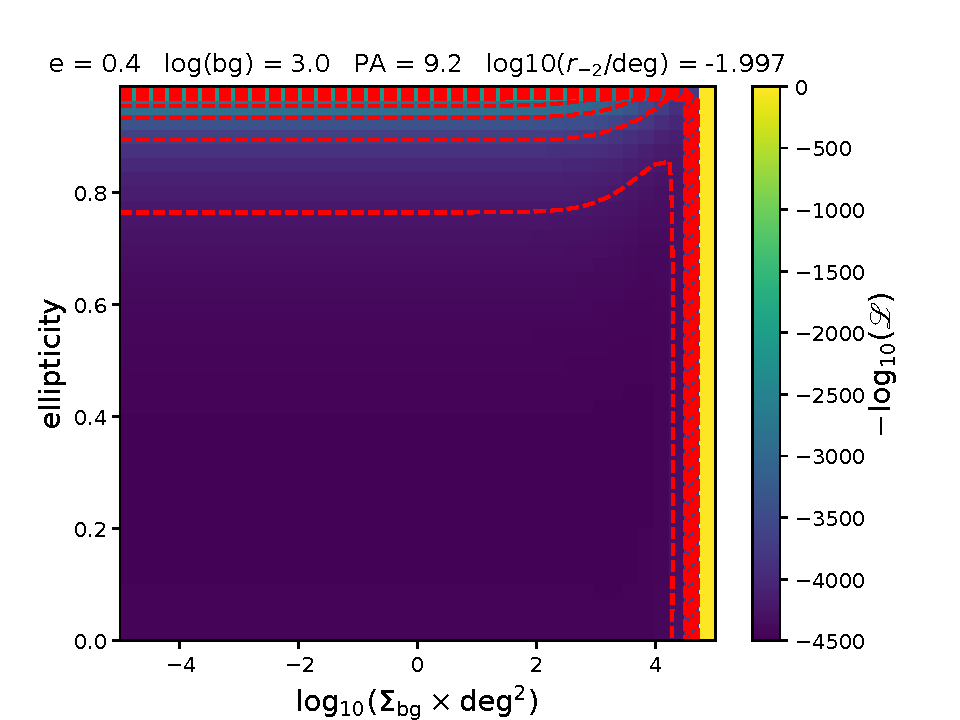
\includegraphics[width=\linewidth]{fixedPA_and_loga.pdf}
		\captionof{figure}{Portion de l'espace des paramètres à PA et $r_{-2}$ fixés. On observe un "mur" au-delà de $\log_{10}(\Sigma_{\rm{bg}}) \sim 4.7$ lorsque la densité surfacique du fond sort des limites imposées. Le HUGE a été ramené à 0 pour des questions de visibilité. Les traits pointillés représentent les courbes d'iso-likelihood.} 
	\end{figure}
	Certains algorithmes comme TNC ou BFGS prennent en compte la gestion des limites sur les paramètres de la fonction à minimiser. Dans ce cas il suffit de fournir pour chaque paramètres un intervalle qui va délimiter l'espace des phases à explorer.\newline
	Par exemple, on n'a aucun intérêt à ce que l'algorithme aille tester des valeurs d'ellipticité hors de l'intervalle $[0,1[$, ou des rayons négatifs.
Au contraire pour certaines méthodes tel que DE ou NM l'espace des paramètres n'est pas restreint et les algorithmes peuvent en principe converger vers un minimum local pour des valeurs de paramètres non-physiques.\newline
	La solution en place au début du stage était de tester les valeurs pour chaque paramètre et de retourner une valeur HUGE (de l'ordre de $10^30$) pour $-\log \mathscr{L}$. En principe cette astuce devrait bien fonctionner pour DE car c'est un algorithme stochastique : en retournant HUGE on force l'algorithme à aller tester de nouvelles solutions ailleurs dans l'espace des paramètres. \newline 
	Pour NM, ce type d'astuce ne fonctionne pas car l'algorithme va rester localisé dans un même zone de l'espace des phases. Si l'algorithme est coincé dans un "mur", en retournant HUGE pour chaque sommet du simplex, l'algorithme ne saura pas dans quelle direction se déplacer. \newline
  La solution à ce problème est de non pas définir un "mur" au niveau du log-likelihood mais d'ajouter une fonction qui va venir le pénaliser de manière continue. Soit $\mathscr{P}$ la fonction pénalité et soit $x \in [x_{\rm{min}} , x_{\rm{max}}]$ un paramètre avec $x_{\rm{min}} ,x_{\rm{max}}$ les valeurs limites. Afin de pénaliser le cas $x < x_{\rm{min}}$ on considère la variable adimensionnée $X = | x/x_{\rm{min}} |$. On souhaite alors que notre fonction pénalité ait les propriétés suivantes:
  \begin{itemize}
    \item $\mathscr{P} \ \ : \ \ ]0,1] \rightarrow \mathbb{R}_+^*$
    \item $\mathscr{P} \xrightarrow{X \rightarrow 0} \infty$
    \item $\mathscr{P} (1) = 0$
    \item $\left. \frac{d\mathscr{P}}{dx} \right | _{x=1} = 0$
  \end{itemize}

  Pour le cas $x > x_{\rm{max}}$ on pose $X = | x/x_{\rm{max}} |$, on peut alors définir la fonction pénalité comme le symétrique selon l'axe $x=1$ de la précédente. \newline
  La fonction pénalité mise en place dans PROF-CL est la suivante
  \begin{equation}
    \mathscr{P}(X) = 
    \begin{cases}    %pour faire un système
      \mathcal{p} (X) & \mbox{si } X = \left | \frac{x}{x_{\rm{min}}} \right | < 1 \\
      \mathcal{p} (2-X) & \mbox{si } X = \left | \frac{x}{x_{\rm{max}}} \right | > 1
    \end{cases}
  \end{equation}
  
  Où on a défini
  \begin{equation}
    \mathcal{p} (X) = 
    \begin{cases}
      \frac{\pi}{2} (X-1) - \tan \left [ \frac{\pi}{2} (X+1) \right ] & \mbox{si } X < 1 \\
      0 & \mbox{si } X > 1
    \end{cases}
  \end{equation}
    
\newpage
\bibliography{ref}  %pour créer ta biblio. avec bibtex (ref est le nom du fichier bibtex)
\bibliographystyle{ieeetr}  %le style de ta biblio.

\newpage
\appendix   %pour commencer les annexes
\section{Solutions analytiques de la densité de surface NFW/NFW tronqué}
  \subsection{NFW circulaire}
	  Pour un profil NFW circulaire, la densité surfacique donnée par la solution de l'équation (\ref{eq:Surface_density}) peut être écrite comme	
  	\begin{equation}
  	  \label{eq:NFW_tilde_tronque}
  		\Sigma_{\rm{NFW}} (R) = \frac{N(r_{-2})}{\pi r_{-2}^2} \tilde{\Sigma}_{\rm{NFW}} (R/r_{-2})
  	\end{equation}
  	La densité surfacique adimensionnée $\tilde{\Sigma}_{\rm{NFW}}$ étant donnée par\cite{Lokas2001}
    \begin{equation}
    	\tilde{\Sigma}_{\rm{NFW}} (X) =  \frac{1 - \rm{C}^{-1} (1/X)/ | X^2 -1 |^{1/2} }{X^2 -1}
    \end{equation}  
    Où l'on a définit
    \begin{equation}
    	\rm{C}^{-1}(Y) = 
    	\begin{cases}  	
    	 	\arccos(Y) & \rm{si} \ \ R>r_{-2}\\
   	  	\arccosh(Y) & \rm{si} \ \ R<r_{-2}
    	\end{cases}
    \end{equation}
  
  \subsection{NFW circulaire tronqué}
    Contrairement aux "mocks académiques" les amas sélectionnés par AMICO pour le Cluster Challenge IV sont tronqués.\newline 
    L'expansion d'Hubble va avoir tendance à décaler les vitesses le long de la ligne de visée des galaxies en arrière plan vers des valeurs positives et celles des galaxies en avant plan vers des valeurs négatives. On peut alors définir la distance maximale selon la ligne de visée par rapport au centre de l'amas noté $r_{\rm{max}}$ comme la distance telle que l'expansion de Hubble soit égale à $\kappa$ fois la dispersion de vitesse de l'amas moyennée dans un disque centré sur l'amas, i.e.
    \begin{equation}
      H_0 r_{\rm{max}} = \kappa \sigma_v
    \end{equation}
    Les amas étant tronqués par AMICO au niveau de la sphère virielle, il est nécessaire quand on calcule la densité surfacique projeté NFW dans l'équation (\ref{eq:Surface_density}) d'effectuer la transformation $\infty \rightarrow r_{\rm{max}}$ au niveau de la borne supérieure.\newline
    Dans le cas considéré ici où $r_{\rm{max}} = r_{\rm{vir}}$ la solution de l'équation (\ref{eq:Surface_density}) avec la nouvelle borne supérieure s'écrit \cite{Mamon2010}
    \begin{equation}
      \Sigma_{\rm{NFW}}^{\rm{trunc}} (R , r_{\rm{vir}}) = \frac{N(r_{-2})}{\pi r_{-2}^2} \tilde{\Sigma}_{\rm{NFW}}^{\rm{trunc}} \left ( \frac{R}{r_{-2}} , c \right )
    \end{equation}
    Où l'on a défini
    \begin{equation}
      \tilde{\Sigma}_{\rm{NFW}}^{\rm{trunc}} ( X, c) = \frac{1}{2 \log 2 - 1}
      \begin{cases}
        \frac{1}{(1-X^2)^{3/2}} \arccosh \left (\frac{c+X^2}{(c+1)X} \right ) - \frac{1}{c+1} \frac{\sqrt{c^2 - X^2}}{1-X^2} & \mbox{si } 0 < X < 1 \\
        \frac{\sqrt{c^2 -1} (c+2)}{3(c+1)^2} + \frac{(2 - c - 4 c^2 - 2 c^3)(X-1)}{5(c+1)^2 \sqrt{c^2 -1}} & \mbox{si } X = 1 \\
        \frac{1}{c+1} \frac{\sqrt{c^2 - X^2}}{X^2-1} - \frac{1}{(X^2-1)^{3/2}} \arccos \left (\frac{c+X^2}{(c+1)X} \right ) & \mbox{si } 1 < X < c \\
        0 & \mbox{si } X = 0 \mbox{ ou } X > c
      \end{cases}
    \end{equation}
\end{document}
